
 \subsection{Vision Computacional \citep*{vc1}}
La visión computacional es un campo de la inteligencia artificial que se enfoca en simular la visión humana y la cognición. Utiliza métodos computacionales y algoritmos para procesar imágenes y videos (incluyendo datos 3D) con el objetivo de:


\begin{itemize}
	\item \textbf{Medir}: Cuantificar características y dimensiones en imágenes.
	\item \textbf{Clasificar}: Identificar y categorizar objetos dentro de las imágenes.
	\item \textbf{Interpretar información visual}: Comprender y derivar significado del contenido visual para crear modelos del mundo real.
\end{itemize}

\begin{figure}[H]
	\begin{center}
		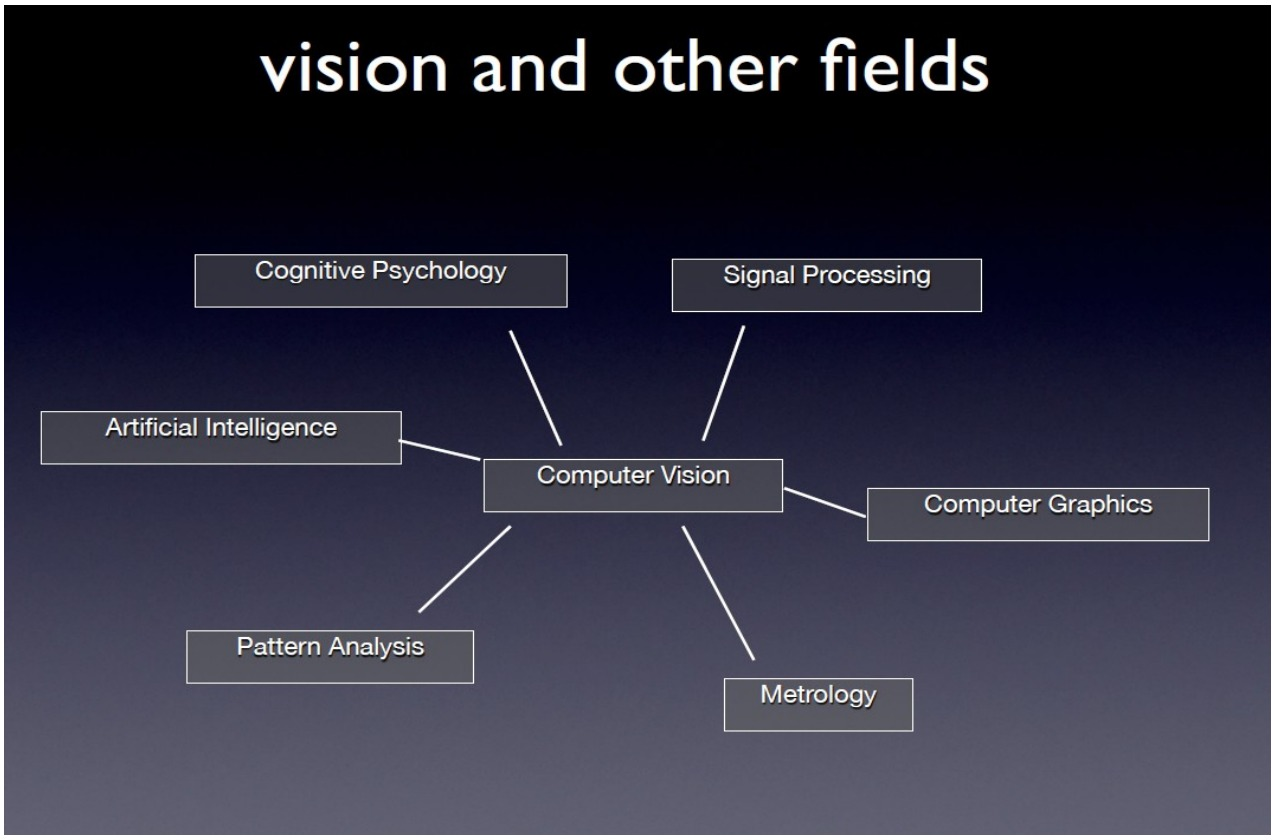
\includegraphics[width=0.8\textwidth]{2/figures/vc1.jpeg}
		\caption{Los otros campos de Vision computacional}
		\label{}
	\end{center}
	
\end{figure}
	
	La visión computacional tiene diversas aplicaciones en múltiples campos:
	
\begin{itemize}
	\item \textbf{Inteligencia Artificial (IA)}: La visión actúa como la etapa de entrada.
	\item \textbf{Medicina}: Estudio de la visión humana y cirugía asistida.
	\item \textbf{Ingeniería y Computación}: Modelado y extracción de modelos.
	\item \textbf{Gráficas}: Generación de contenido y creación.
\end{itemize}
	
\subsubsection{¿Para qué estudiamos Visión Computacional?}
	
El objetivo de la visión computacional (VC) es hacer juicios prácticos sobre objetos físicos del mundo real (escenas) a partir de imágenes digitales capturadas.

Por lo tanto, la tarea de la VC implica crear descriptores de la escena basados en características relevantes encontradas en una imagen..
	
	
\subsubsection{Modelo de Imagen “Pinhole”}
	
La proyección de perspectiva puede producir imágenes invertidas. En algunas situaciones, es beneficioso tener en cuenta la imagen virtual asociada con el plano situado frente al "pinhole", a la misma distancia que el plano de la imagen, dependiendo del contexto.

	
\begin{figure}[H]
	\begin{center}
		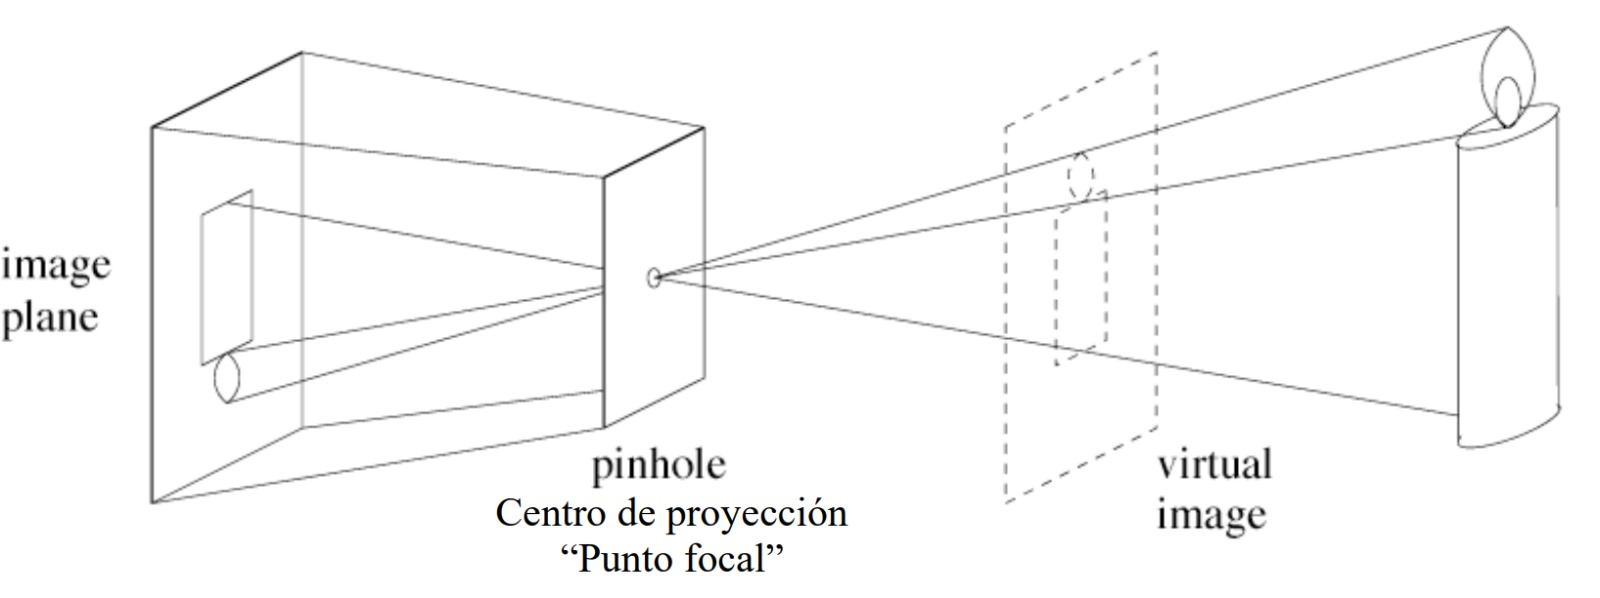
\includegraphics[width=0.8\textwidth]{2/figures/vc2.jpeg}
		\caption{Modelo pinhole}
		\label{}
	\end{center}
	
\end{figure}


\subsubsection{Efectos de Perspectiva}




\begin{figure}[H]
	\begin{center}
		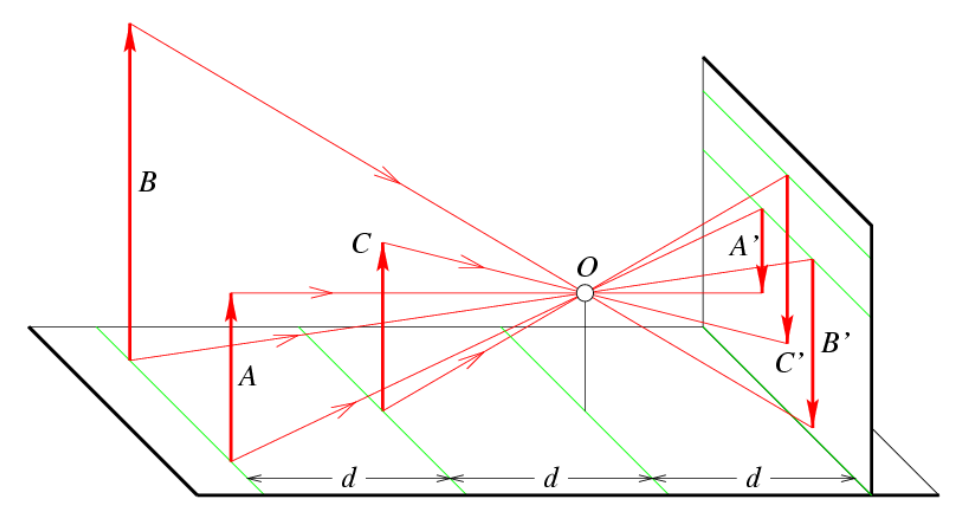
\includegraphics[width=0.8\textwidth]{2/figures/vc3.png}
		\caption{Efectos de Perspectiva}
		\label{}
	\end{center}
	
\end{figure}

\begin{itemize}
	\item \textbf{Tamaño Aparente}: Líneas C' y B' simulan ser similares en cuanto a grandeza, por otro lado, C = ½ B ya que la distancia de B a O es 2d y la distancia de C a O es d.
	\item \textbf{Punto de Fuga}: Las líneas paralelas en la escena se encuentran en un objetivo de fuga en la imagen, que es la intersección de las rectas paralelas en el panorama.
\end{itemize}


\subsubsection{Metodos de Proyección}

\paragraph{Simulacion de la visoon humana }

\begin{itemize}
	\item Proyección de perspectiva débil: Esta paráfrasis enfatiza que la proyección en perspectiva débil da como resultado una distorsión mínima de los tamaños relativos de los objetos en la escena.
	\item Proyección ortográfica: Se dice que la cámara se encuentra a una distancia continua de la escena, con rayos paralelos al eje ocular y ortogonales al plano de proyección.
\end{itemize}


\subsubsection{Aberraciones}

\begin{itemize}
	\item \textbf{Geométricas}: Incluyen aberraciones esféricas, astigmatismo y distorsión.
	\item \textbf{Cromáticas}: Dependen de la longitud de onda de la luz.
\end{itemize}

\paragraph{Tipos de Aberraciones Geométricas}

\begin{itemize}
	\item Aberraciones esféricas: Los rayos exteriores tienden a converger en una posición distinta a los rayos más internos, creando un círculo de confusión.
	\item Astigmatismo: Diferente distancia focal para rayos inclinados.
	\item Distorsión: Puede ser corregida si se conocen los parámetros. Se presenta como distorsión en cojín (tele-foto) o en barril (gran-angular).
\end{itemize}

	

\subsubsection{¿Qué es una imagen?}

\begin{itemize}
	\item \textbf{Definición}: Una imagen es una matriz de valores organizada en dos dimensiones, que usualmente representa la intensidad de la radiación electromagnética
	\item \textbf{Características}:
	\begin{itemize}
		\item \textbf{Muestreo espacial}
		\item \textbf{Cuantización numérica}: Ejemplo, Negro = 0, Blanco = 255.
		\item \textbf{Cuantización espectral}
	\end{itemize}
\end{itemize}

\subsubsection{Representación del Color}

\begin{itemize}
	\item \textbf{Motivación}:
	\begin{itemize}
		\item En análisis automático, el color ayuda en la detección de objetos y en la caracterización de escenas.
		\item En el análisis humano, el color posibilita la diferenciación de una gama más amplia de matices e intensidades en contraste con los niveles de gris.
	\end{itemize}
	\item \textbf{Fundamentos del color}: 
	\begin{itemize}
		\item La luz blanca se divide en un espectro de color con seis regiones: violeta, azul, verde, amarillo, naranja y rojo.
		\item Los colores percibidos están determinados por la naturaleza de la luz reflejada por los objetos.
		\item La luz visible es una banda estrecha del espectro electromagnético.
	\end{itemize}
	\item \textbf{Síntesis aditiva}: Los colores se suman (objetos luminosos).
	\item \textbf{Síntesis sustractiva}: Los colores se restan (pigmentos).
\end{itemize}
	\begin{figure}[H]
	\begin{center}
		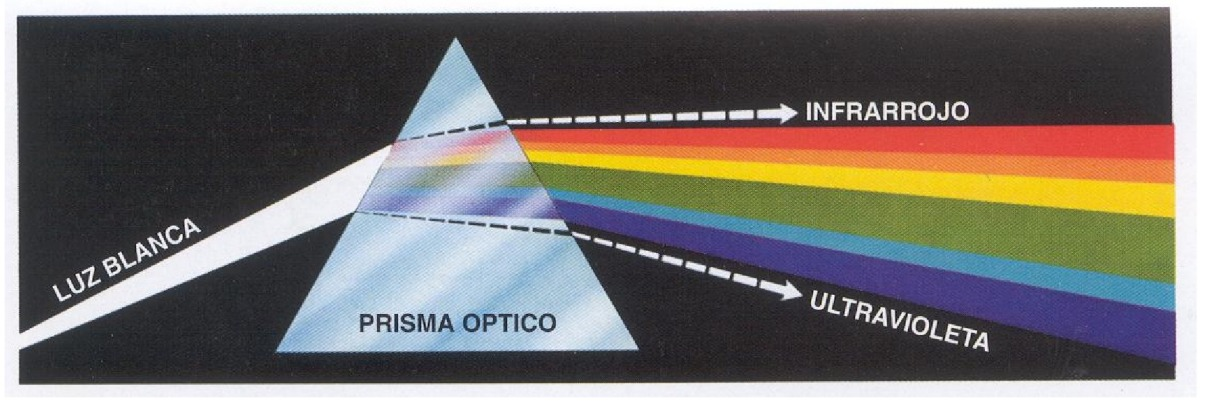
\includegraphics[width=0.8\textwidth]{2/figures/vc6.jpeg}
		\caption{La luz blanca se divide en un espectro de color que contiene
			6 regiones: violeta, azul, verde, amarillo, naranja y rojo.}
		\label{}
	\end{center}
	
\end{figure}

 \subsection{Rancha "Phytohpthora Infestans" Tizon Tardio \citep*{prom2}}
 
 El cultivo de papa es esencial para la seguridad alimentaria mundial, pero enfrenta desafíos por enfermedades como el tizón tardío, causado por Phytophthora infestans. Este patógeno puede causar pérdidas significativas en la producción y afecta A todas las fases de desarrollo de la planta. Se han desarrollado diversas estrategias de manejo, incluyendo el control químico y cultural, pero se requiere un enfoque integrado para su control efectivo. Esta revisión se centra en la prevalencia, ciclo de vida y estrategias de manejo del tizón tardío.
 
 \subsubsection{Introduccion}
 La papa (Solanum tuberosum L.) es un cultivo significativo, especialmente en Europa y Asia, donde más del 80\% de la producción mundial se concentra. China es el mayor productor mundial de papas, seguido por Rusia e India. Sin embargo, enfermedades como el tizón tardío, causado por Phytophthora infestans, representan una amenaza seria para la producción. Esta enfermedad puede causar pérdidas considerables y afecta todas las etapas de crecimiento de la planta, incluyendo los tubérculos, lo que puede llevar a una pérdida del 100\% de la producción. Las estrategias de manejo, como el control químico y cultural, son importantes para su control. La tizón tardío es especialmente devastador en áreas donde la papa es un alimento básico, como en Etiopía, donde puede causar pérdidas del 31 al 100\%. A nivel mundial, se estima que la enfermedad causa pérdidas anuales de hasta 5 mil millones de dólares, y ha tenido un impacto significativo en eventos históricos, como la Gran Hambruna Irlandesa en la década de 1840.
 
  \subsubsection{Ciclo de vida y epidemiología del tizón tardío}
  El tizón tardío en los campos de papa comienza con la aparición de lesiones pequeñas, irregulares y de color verde claro a oscuro que exudan agua. Estas generalmente comienzan en las hojas inferiores y se propagan rápidamente en ambientes húmedos, formando áreas marrones deterioradas con bordes irregulares. Un crecimiento miceliar blanco y mohoso se desarrolla alrededor de las lesiones en la superficie interna de las hojas. La infección puede matar y dañar hojas enteras, y el micelio crece profusamente entre las células del hospedero, causando lesiones de color verde marrón o amarillento que eventualmente se vuelven negras. La enfermedad puede persistir en plantas de papa, suelo, tubérculos infectados y tubérculos voluntarios que sobreviven el invierno. Los esporangios de Phytophthora infestans pueden dispersarse por el viento, la precipitación, el transporte mecánico y los animales, promoviendo la transmisión de la enfermedad. La enfermedad se desarrolla rápidamente en condiciones húmedas y temperaturas entre 15 y 25 °C, y puede causar la muerte de plantas enteras en pocos días o semanas.
  
   \subsubsection{Phytophthora infestans - Síntomas de la enfermedad, Modo de infección y propagación}
 Phytophthora infestans, un patógeno vegetal diploide, comparte rasgos comunes con los hongos y se reproduce asexualmente mediante esporangios con forma de limón que se propagan a través de mecanismos mecánicos, del viento y de la lluvia. Los zoosporos se forman en condiciones húmedas y frescas, mientras que los esporangios germinan en ambientes secos y cálidos. La reproducción sexual puede ocurrir entre hifas compatibles, lo que resulta en la producción de oosporos, que pueden sobrevivir en el suelo hasta por cuatro años. Tanto la reproducción asexual como la sexual contribuyen a la capacidad del patógeno para infectar nuevas plantas. Los esporangios, zoosporos u oosporos acceden a los tejidos de las plantas huésped a través de los estomas o áreas lesionadas, donde estructuras especializadas llamadas haustorios ayudan en la absorción de nutrientes. El desarrollo de esporangios en esporangióforos conduce a la esporulación, con esporangios transportados por el aire hacia plantas sanas. La infección exitosa implica interacciones complejas entre el patógeno, el huésped y el medio ambiente, influenciadas por factores como la humedad, la temperatura, la virulencia del patógeno y la resistencia del huésped, lo que conduce a pérdidas agrícolas significativas.
 
 	\begin{figure}[H]
 	\begin{center}
 		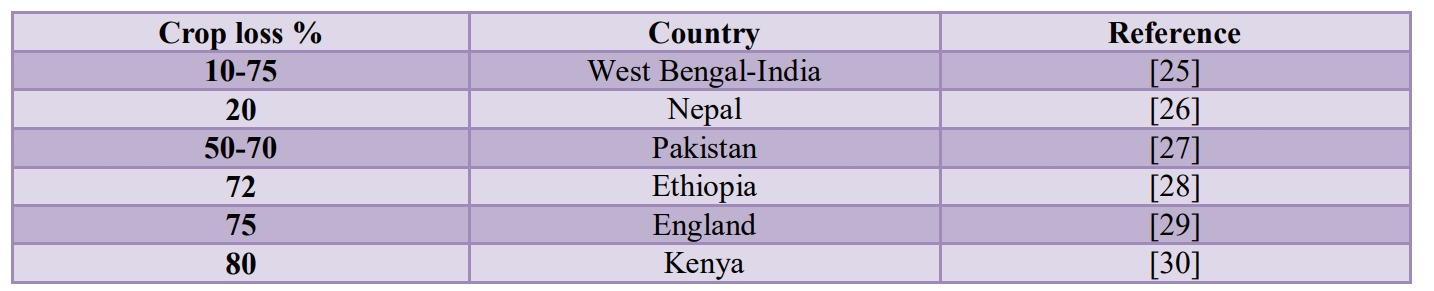
\includegraphics[width=0.8\textwidth]{2/figures/prom1.jpeg}
 		\caption{Pérdida de cosechas a nivel nacional debido al tizón tardío de la papa}
 		\label{}
 	\end{center}
 	
 \end{figure}
 
    \subsubsection{Conclusion}
    El enfoque herbal ha mostrado promesa en la búsqueda de extractos vegetales con acción anti-oomycete, demostrando eficacia contra P. infestans. Algunas de estas sustancias han resultado tan efectivas como los fungicidas sintéticos en la prevención del crecimiento de P. infestans in vitro o en la reducción de la gravedad del tizón tardío en plantas hospederas. La resistencia de las plantas hospederas al patógeno puede ofrecer beneficios económicos a largo plazo para los agricultores y reducir las alteraciones en la estructura poblacional de P. infestans, lo que disminuye el potencial de resistencia a los fungicidas. Sin embargo, dado que no existe un método de manejo único que sea efectivo en todo el mundo debido a la introducción de nuevas cepas, es crucial desarrollar nuevos enfoques para tratar esta enfermedad y superar el problema de la resistencia.